\documentclass[notitlepage]{article}

\usepackage[portuges]{babel}
\usepackage[utf8]{inputenc}
\usepackage{amsmath}
\usepackage{titlesec}
\usepackage{indentfirst}
\usepackage{graphicx}
\usepackage{multicol,lipsum}
\usepackage{times}
\usepackage[top=2.5cm, bottom=2.5cm, left=3cm, right=3cm]{geometry}
\usepackage{setspace}
\usepackage{etex}
\usepackage{tabto}

\addto\captionsportuges{% Replace "english" with the language you use
  \renewcommand{\contentsname}%
    {13\hspace{4.25mm} Índice}%
}

\begin{document}
%\maketitle
\begin{flushright}
    \begin{bfseries}
        \Huge{Modelo de Casos de Uso - Projeto Parte 2}\\
    \end{bfseries}
    \rule{16cm}{3pt}\vskip1cm
\end{flushright}

	\begin{center}
		\large{Universidade Federal de São Carlos}\\
		\large{Introdução a Sistemas de Informação}\\ 
		\large{Professora Dra. Sandra Fabbri}\\
		\large{São Carlos, SP - Brasil, 05/2017}\\
        \vspace{45pt}
        \textbf{\LARGE{Projeto: Sistema de Gerenciamento de Hotel}}\\
		\vspace{1,5cm}
	\end{center}
	
	\begin{flushleft}
		\begin{tabbing}
		Bruna Zamith Santos, 628093\\
		Guilherme Nishi Kanashiro, 628298\\
		Henrique Frajacomo, 726536\\
		Leonardo Utida Alcantara, 628182\\
		Rodolfo Krambeck Asbahr, 628042\\
		Tiago Bachiega de Almeida, 628247
	\end{tabbing}
 \end{flushleft}
	\vspace{1cm}
\nopagebreak


\clearpage
\section{Diagrama de MCU}
\begin{figure}[!htbp]
	\centering
  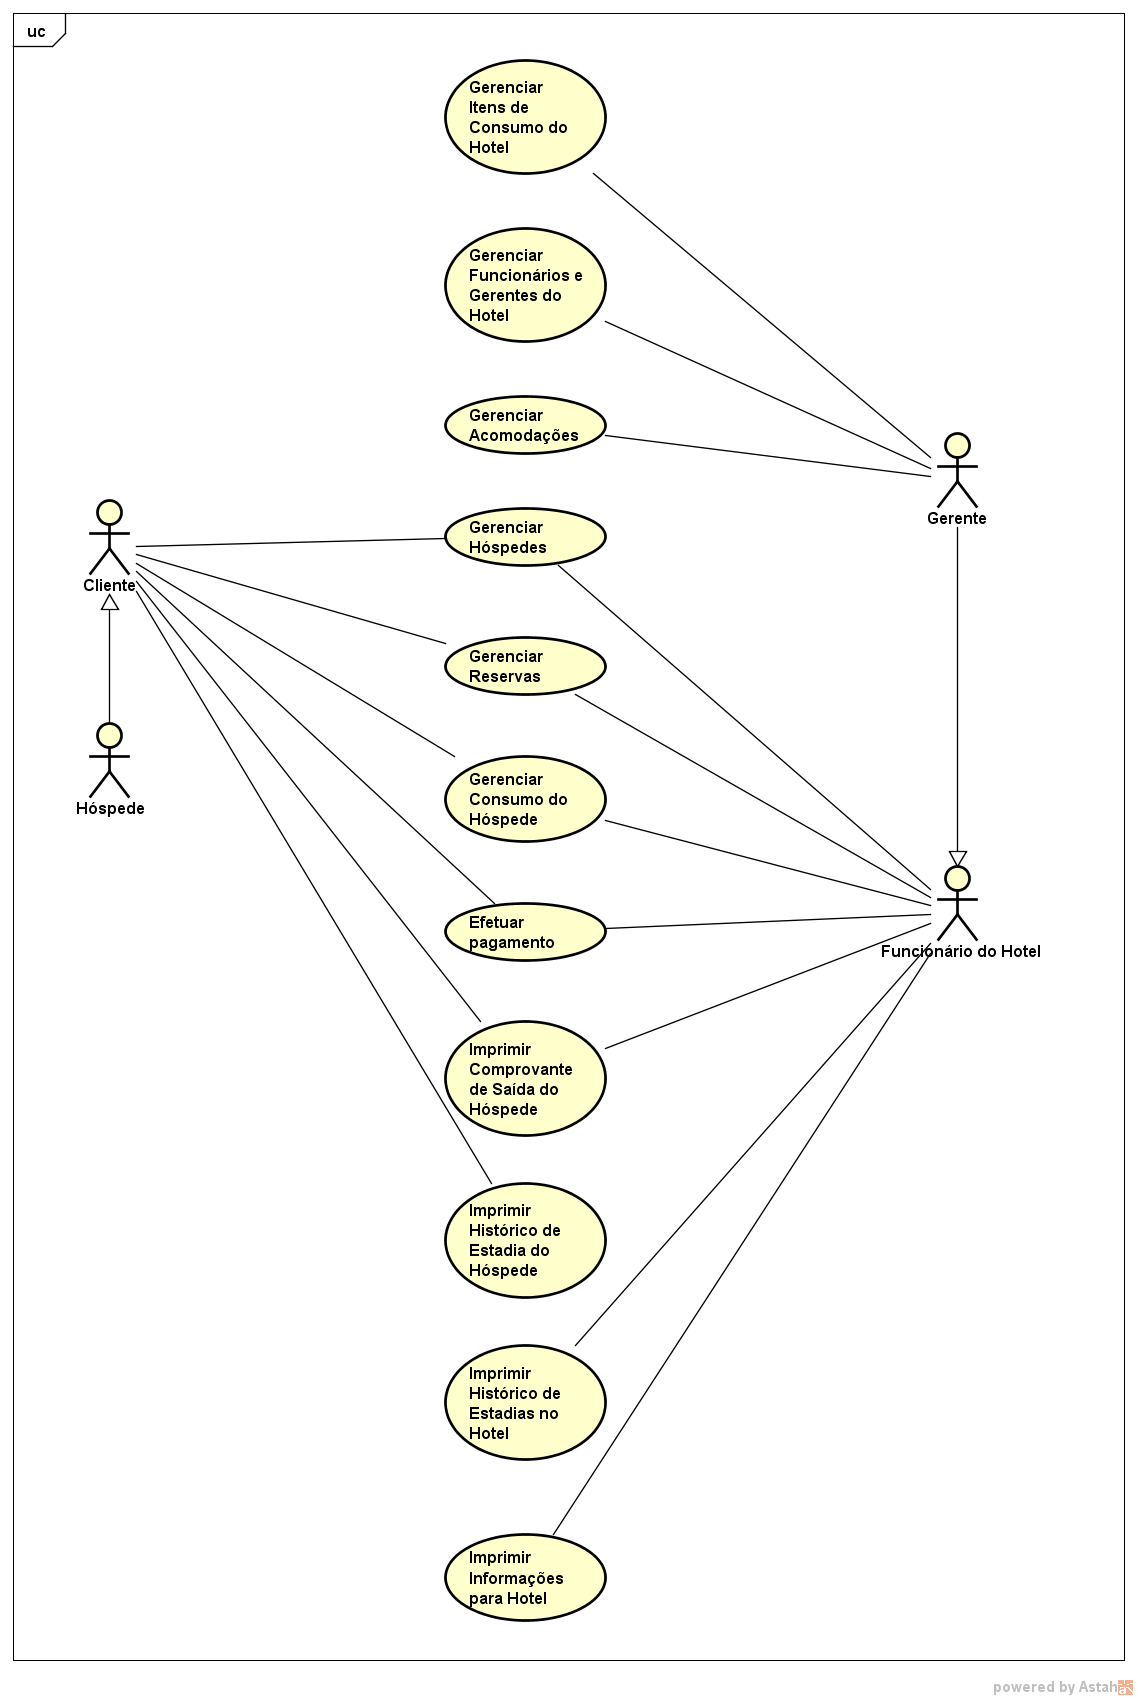
\includegraphics[scale=0.45]{MCU.png}
  \caption{Diagrama de MCU}
  \label{fig:MCU}
\end{figure}

\clearpage

\section{ID: UC1}
\noindent\textbf{Caso de uso}: Gerenciar Hóspedes.\\
\textbf{Atores Primários}: Cliente. \\
\textbf{Atores Secundários}: Funcionário do Hotel.\\
\textbf{Propósito}: Incluir, Alterar, Remover, Fazer Check-in e/ou Fazer Check-Out do Hotel.\\
\textbf{Visão Geral}: O Funcionário do Hotel acessa um painel onde pode incluir dados do cliente, alterá-los ou removê-los.Além disso, efetua o check-in e o check-out do cliente.\\
\textbf{Pré-condições}: O funcionário já estar cadastrado no sistema.\\
\textbf{Pós-condições}: Um novo hóspede é incluído, removido ou alterado no sistema.\\
\textbf{Referências Cruzadas}: R.1, R.7, R.20, R.21, R.22, R.23\\
\newline
\textbf{Fluxo Principal}:\\

\begin{table}[!htbp]
\centering
\label{UC1}
\resizebox{\textwidth}{!}{%
\begin{tabular}{|p{8cm}|p{8cm}|}
\hline
\textbf{Ação do Ator}                                      & \textbf{Resposta do Sistema}                                                                           \\ \hline
1. O Funcionário do Hotel acessa o sistema.                & 2. Exibe a tela de login, solicitando email e senha do Funcionário do Hotel.                           \\ \hline
3. O Funcionário do Hotel insere seu email e senha.        & 4. Verifica os dados de login.                                                                         \\ \hline
                                                           & 5. Exibe o Menu Principal.                                                                             \\ \hline
6. O Funcionário do Hotel seleciona a opção “Gerenciar Hóspedes”.    & 7. Exibe a tela com as opções Incluir, Alterar, Remover, Fazer Check-in e Fazer Check-out de Clientes. \\ \hline
8. O Funcionário do Hotel seleciona a opção “Incluir”.     & 9. Exibe a tela de inclusão de dados do Hóspede, com campos de preenchimento específicos.             \\ \hline
10. O Funcionário do Hotel preenche os campos com dados do Cliente, como especificado no requisito 1. & 11. Exibe a tela informando que a operação foi realizada com sucesso.                                  \\ \hline
                                                           & 12. Exibe o Menu Principal novamente (Passo 5).                                                        \\ \hline
\end{tabular}%
}
\end{table}

\textbf{Fluxos Alternativos}:\\
\begin{itemize}
\item \underline{Passo 2}: O Funcionário do Hotel já está logado, então avança para o Passo 5.
\item \underline{Passo 4}: O Funcionário do Hotel insere email e/ou senha incorretos. O sistema exibe a tela informando que os dados de login são inválidos, então retorna para o Passo 2.
\item \underline{Passos 2 - 10}: O Funcionário do Hotel deseja encerrar o sistema e cancelar a operação atual, selecionando a opção de fechar o navegador. O sistema é encerrado e nenhuma informação é salva. 
\item \underline{Passos 8 - 10}: O Funcionário do Hotel seleciona a opção “Remover”. O sistema exibe um campo de busca pelo nome do Cliente. O Funcionário do Hotel seleciona o Cliente a ser removido, e seus dados são deletados do sistema.  
\item \underline{Passos 8 - 10}: O Funcionário do Hotel seleciona a opção “Alterar”; o sistema exibe um campo de busca pelo nome do Cliente. O Funcionário do Hotel seleciona o Cliente a ser alterado, e seus dados previamente preenchidos são exibidos. O Funcionário do Hotel seleciona os dados a serem alterados, modifica-os e então clica em “Salvar”. Os dados do Cliente são atualizados no sistema.
\item \underline{Passos 8 - 10}: O Funcionário do Hotel seleciona a opção “Fazer Check-in”, o sistema exibe um campo de busca pelo nome do Cliente. O Funcionário do Hotel seleciona o Cliente que deseja fazer check-in. O Sistema exibe uma tela informando a entrada de dados como data e hora do check-in. O Funcionário do Hotel clica em “Salvar”. 
\item \underline{Passos 8 - 10}: O Funcionário do Hotel seleciona a opção “Fazer Check-out”, o sistema exibe um campo de busca pelo nome do Cliente. O Funcionário do Hotel seleciona o Cliente que deseja fazer check-out. O Sistema exibe uma tela informando a entrada de dados como data e hora do check-out. O Funcionário do Hotel clica em “Salvar”. 
\item \underline{Passo 10}: O Funcionário do Hotel insere dados que já estão cadastrados no sistema. O sistema exibe na tela a informação de que o Cliente já está cadastrado, então retorna para o Passo 5.
\item \underline{Passo 10}: O Funcionário do Hotel não preenche todos os dados obrigatórios. O sistema exibe na tela a informação de quais dados estão faltando, então retorna para o Passo 9.

\end{itemize}

\begin{figure}[!htbp]
	\centering
  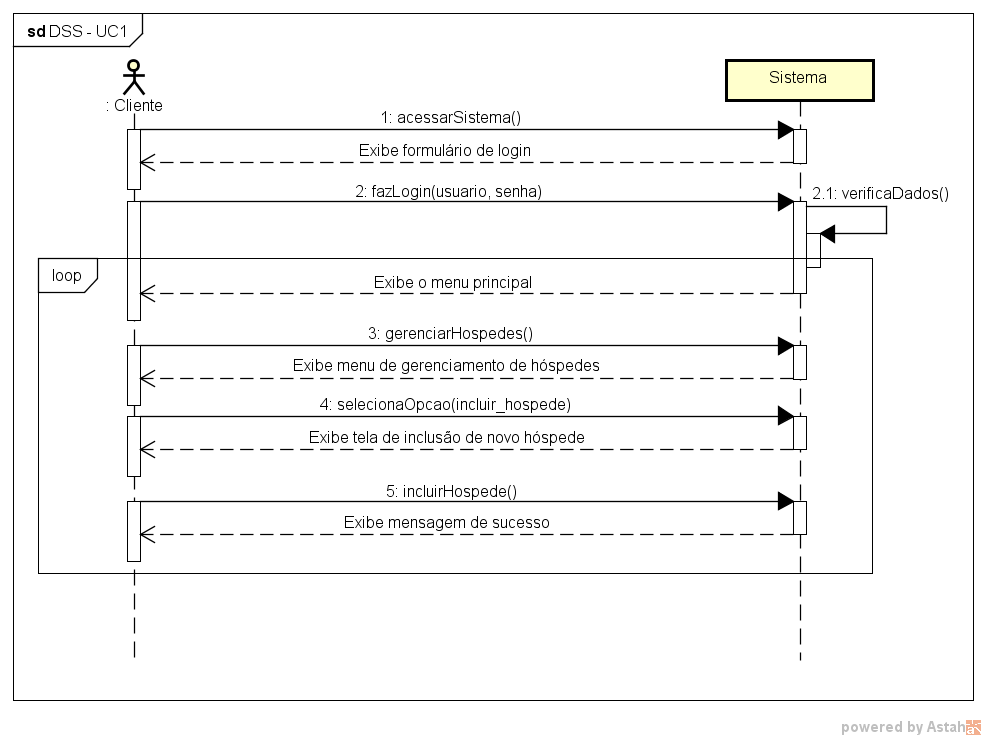
\includegraphics[scale=0.65]{UC1.png}
  \caption{DSS do UC1}
  \label{fig:UC1}
\end{figure}

\clearpage

\section{ID: UC2}
\noindent\textbf{Caso de uso}: Gerenciar Itens de Consumo do Hotel.\\
\textbf{Atores Primários}: Gerente do Hotel (Administrador do Sistema). \\
\textbf{Atores Secundários}: \\
\textbf{Propósito}: Incluir, Alterar e/ou Remover os Itens de Consumo Disponíveis no Hotel.\\
\textbf{Visão Geral}: O Gerente do Hotel (administrador) acessa um painel onde pode incluir, alterar ou remover itens de consumo.\\
\textbf{Pré-condições}: O Gerente do Hotel (administrador) já estar cadastrado no sistema.\\
\textbf{Pós-condições}: Um novo item de consumo é incluído, removido ou alterado no sistema.\\
\textbf{Referências Cruzadas}: R.2, R.20, R.22, R.23\\
\newline
\textbf{Fluxo Principal}:\\

\begin{table}[!htbp]
\centering
\label{UC2}
\resizebox{\textwidth}{!}{%
\begin{tabular}{|p{8cm}|p{8cm}|}
\hline
\textbf{Ação do Ator}                                      & \textbf{Resposta do Sistema}                                                                           \\ \hline
1. O Gerente do Hotel acessa o sistema.                & 2. Exibe tela de login, solicitando email e senha do Gerente do Hotel.                           \\ \hline
3. Gerente do Hotel insere seu email e senha.        & 4. Verifica os dados de login.                                                                         \\ \hline
                                                           & 5. Exibe o Menu Principal.                                                                             \\ \hline
6. O Gerente do Hotel seleciona a opção “Gerenciar Itens de Consumo do Hotel”.
    & 7. Exibe a tela com as opções Incluir, Alterar ou Remover Itens de Consumo do Hotel. \\ \hline
8. O Gerente do Hotel seleciona a opção “Incluir”.     & 9. Exibe a tela de inclusão de Itens de Consumo do Hotel, com campos de preenchimento específicos.             \\ \hline
10. O Gerente do Hotel preenche os campos com dados do Item de Consumo, como especificado no requisito 2. & 11. Exibe a tela informando que a operação foi realizada com sucesso.                                  \\ \hline
                                                           & 12. Exibe o Menu Principal novamente (Passo 5).                                                        \\ \hline
\end{tabular}%
}
\end{table}

\textbf{Fluxos Alternativos}:\\
\begin{itemize}
\item \underline{Passo 2}: O Gerente do Hotel já está logado, então avança para o Passo 5.
\item \underline{Passo 4}: O Gerente do Hotel insere email e/ou senha incorretos. O sistema exibe a tela informando que os dados de login são inválidos, então retorna para o Passo 2.
\item \underline{Passos 2 - 10}: O Gerente do Hotel deseja encerrar o sistema e cancelar a operação atual, selecionando a opção de fechar o navegador. O sistema é encerrado e nenhuma informação é salva.  
\item \underline{Passos 8 - 10}: O Gerente do Hotel seleciona a opção “Remover”. O sistema exibe um campo de busca pelo item de consumo. O Gerente do Hotel seleciona o item a ser removido, e o dado é removido do sistema.    
\item \underline{Passos 8 - 10}: O Gerente do Hotel seleciona a opção “Alterar”; o sistema exibe um campo de busca pelo item de consumo. O Gerente do Hotel seleciona o item a ser alterado, e seus dados previamente preenchidos são exibidos. O Gerente do Hotel seleciona os dados a serem alterados, modifica-os e então clica em “Salvar”. Os dados do item são atualizados no sistema.
\item \underline{Passo 10}: O Gerente do Hotel insere dados que já estão cadastrados no sistema. O sistema exibe na tela a informação de que o item já está cadastrado, então retorna para o Passo 5.
\item \underline{Passo 10}: O Gerente do Hotel não preenche todos os dados obrigatórios. O sistema exibe na tela a informação de quais dados estão faltando, então retorna para o Passo 9.

\end{itemize}

\begin{figure}[!htbp]
	\centering
  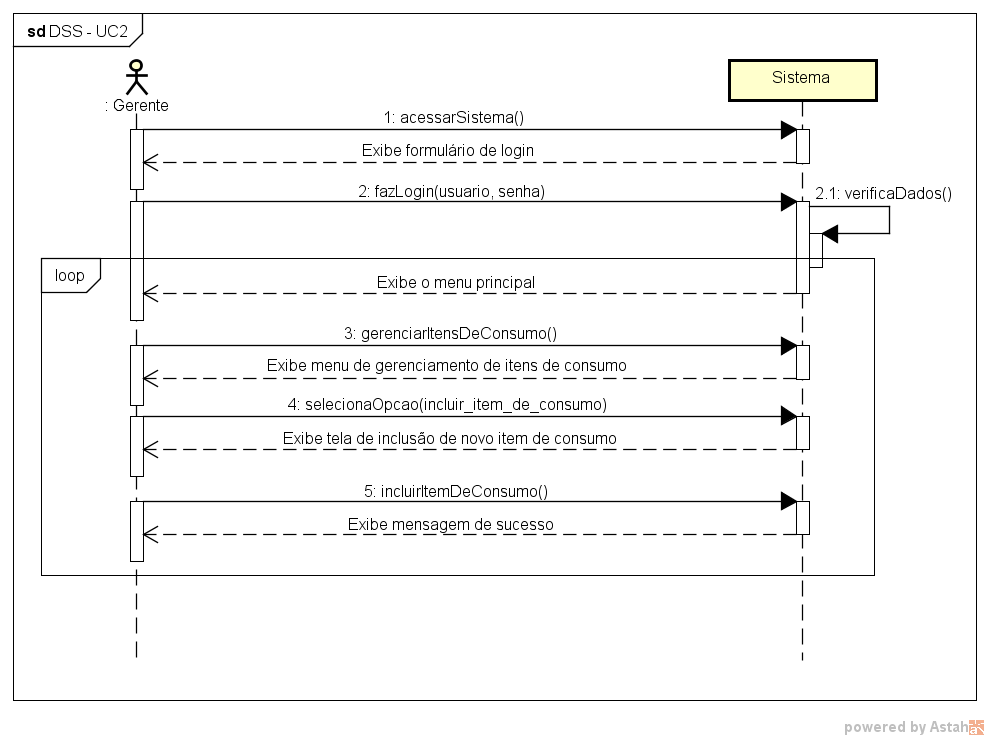
\includegraphics[scale=0.65]{UC2.png}
  \caption{DSS do UC2}
  \label{fig:UC2}
\end{figure}

\clearpage

\section{ID: UC3}
\noindent\textbf{Caso de uso}: Gerenciar Funcionários e Gerentes do Hotel.\\
\textbf{Atores Primários}: Gerente do Hotel (Administrador do Sistema). \\
\textbf{Atores Secundários}: \\
\textbf{Propósito}: Incluir, Alterar e/ou Remover Dados de Funcionários e Gerentes do Hotel.\\
\textbf{Visão Geral}: O Gerente do Hotel (administrador) acessa um painel onde pode incluir, alterar ou remover dados de funcionários e gerentes do hotel.\\
\textbf{Pré-condições}: O Gerente do Hotel (administrador) já estar cadastrado no sistema.\\
\textbf{Pós-condições}: Um novo funcionário ou gerente é incluído, removido ou alterado no sistema.\\
\textbf{Referências Cruzadas}: R.3, R.20, R.21, R.22, R.23\\
\newline
\textbf{Fluxo Principal}:\\

\begin{table}[!htbp]
\centering
\label{UC3}
\resizebox{\textwidth}{!}{%
\begin{tabular}{|p{8cm}|p{8cm}|}
\hline
\textbf{Ação do Ator}                                      & \textbf{Resposta do Sistema}                                                                           \\ \hline
1. O Gerente do Hotel acessa o sistema.                & 2. Exibe tela de login, solicitando email e senha do Gerente do Hotel.                           \\ \hline
3. Gerente do Hotel insere seu email e senha.        & 4. Verifica os dados de login.                                                                         \\ \hline
                                                           & 5. Exibe o Menu Principal.                                                                             \\ \hline
6. O Gerente do Hotel seleciona a opção “Gerenciar Funcionários e Gerentes do Hotel”.
    & 7. Exibe a tela com as opções Incluir, Alterar ou Remover Funcionários e Gerentes do Hotel. \\ \hline
8. O Gerente do Hotel seleciona a opção “Incluir”.     & 9. Exibe a tela de inclusão de dados do Funcionário ou Gerente, com campos de preenchimento específicos.             \\ \hline
10. O Gerente do Hotel preenche os campos com dados do Funcionário ou Gerente, como especificado no requisito 3. & 11. Exibe a tela informando que a operação foi realizada com sucesso.                                  \\ \hline
                                                           & 12. Exibe o Menu Principal novamente (Passo 5).                                                        \\ \hline
\end{tabular}%
}
\end{table}

\textbf{Fluxos Alternativos}:\\
\begin{itemize}
\item \underline{Passo 2}: O Gerente do Hotel já está logado, então avança para o Passo 5.
\item \underline{Passo 4}: O Gerente do Hotel insere email e/ou senha incorretos. O sistema exibe a tela informando que os dados de login são inválidos, então retorna para o Passo 2.
\item \underline{Passos 2 - 10}: O Gerente do Hotel deseja encerrar o sistema e cancelar a operação atual, selecionando a opção de fechar o navegador. O sistema é encerrado e nenhuma informação é salva.  
\item \underline{Passos 8 - 10}: O Gerente do Hotel seleciona a opção “Remover”. O sistema exibe um campo de busca pelo nome do Funcionário ou Gerente. O Gerente do Hotel seleciona o Funcionário ou Gerente a ser removido, e seus dados são deletados do sistema.    
\item \underline{Passos 8 - 10}: O Gerente do Hotel seleciona a opção “Alterar”; o sistema exibe um campo de busca pelo nome do Funcionário ou Gerente. O Gerente do Hotel seleciona o Funcionário ou Gerente a ser alterado, e seus dados previamente preenchidos são exibidos. O Gerente do Hotel seleciona os dados a serem alterados, modifica-os e então clica em “Salvar”. Os dados do Funcionário ou Gerente são atualizados no sistema.
\item \underline{Passo 10}: O Gerente do Hotel insere dados que já estão cadastrados no sistema. O sistema exibe na tela a informação de que o Funcionário ou Gerente já está cadastrado, então retorna para o Passo 5.
\item \underline{Passo 10}: O Gerente do Hotel não preenche todos os dados obrigatórios. O sistema exibe na tela a informação de quais dados estão faltando, então retorna para o Passo 9.

\end{itemize}

\begin{figure}[!htbp]
	\centering
  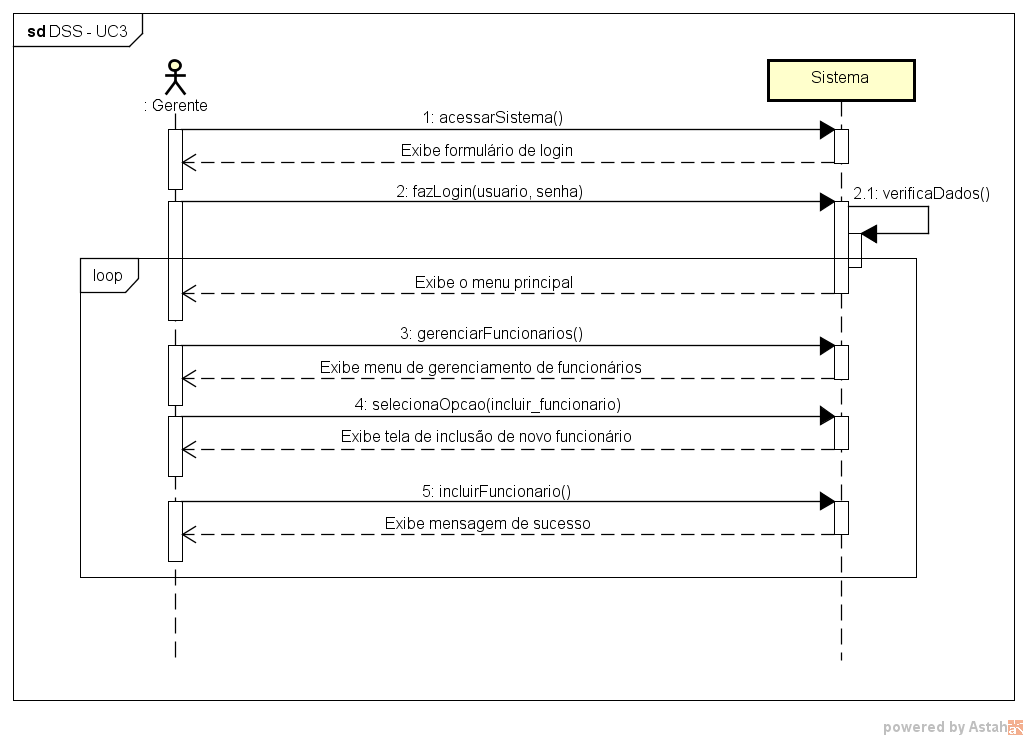
\includegraphics[scale=0.65]{UC3.png}
  \caption{DSS do UC3}
  \label{fig:UC3}
\end{figure}


\clearpage

\section{ID: UC4}
\noindent\textbf{Caso de uso}: Gerenciar Acomodações.\\
\textbf{Atores Primários}: Gerente do Hotel (Administrador do Sistema). \\
\textbf{Atores Secundários}: \\
\textbf{Propósito}: Incluir, Alterar e/ou Remover Tipos de Acomodações e Acomodações do Hotel.\\
\textbf{Visão Geral}: O Gerente do Hotel (administrador) acessa um painel onde pode incluir, alterar ou remover os tipos de acomodações do hotel. Além disso, pode incluir, alterar ou remover as acomodações do hotel.\\
\textbf{Pré-condições}: O Gerente do Hotel (administrador) já estar cadastrado no sistema.\\
\textbf{Pós-condições}: Um novo tipo de acomodação ou acomodação é incluído, removido ou alterado no sistema.\\
\textbf{Referências Cruzadas}: R.4, R.5, R.20, R.22, R.23\\
\newline
\textbf{Fluxo Principal}:\\

\begin{table}[!htbp]
\centering
\label{UC4}
\resizebox{\textwidth}{!}{%
\begin{tabular}{|p{8cm}|p{8cm}|}
\hline
\textbf{Ação do Ator}                                      & \textbf{Resposta do Sistema}                                                                           \\ \hline
1. O Gerente do Hotel acessa o sistema.                & 2. Exibe tela de login, solicitando email e senha do Gerente do Hotel.                           \\ \hline
3. O Gerente do Hotel insere seu email e senha.        & 4. Verifica os dados de login.                                                                         \\ \hline
                                                           & 5. Exibe o Menu Principal.                                                                             \\ \hline
6. O Gerente do Hotel seleciona a opção “Gerenciar Acomodações”.
    & 7. Exibe a tela com as opções Incluir, Alterar ou Remover Tipos de Acomodações ou Acomodações do Hotel. \\ \hline
8. O Gerente do Hotel seleciona a opção “Incluir”.     & 9. Exibe a tela com as opções "Tipo de Acomodação" ou "Acomodação"\\ \hline
10. O Gerente do Hotel seleciona a opção "Tipo de Acomodação". & 11. Exibe a tela de inclusão de dados de Tipo de Acomodação, com campos de preenchimento específicos.             \\ \hline
12. O Gerente do Hotel preenche os campos com dados do tipo de acomodação, como especificado no requisito 4. & 13. Exibe a tela informando que a operação foi realizada com sucesso.                                  \\ \hline
                                                           & 14. Exibe o Menu Principal novamente (Passo 5).                                                        \\ \hline
\end{tabular}%
}
\end{table}

\textbf{Fluxos Alternativos}:\\
\begin{itemize}
\item \underline{Passo 2}: O Gerente do Hotel já está logado, então avança para o Passo 5.
\item \underline{Passo 4}: O Gerente do Hotel insere email e/ou senha incorretos. O sistema exibe a tela informando que os dados de login são inválidos, então retorna para o Passo 2.
\item \underline{Passos 2 - 12}: O Gerente do Hotel deseja encerrar o sistema e cancelar a operação atual, selecionando a opção de fechar o navegador. O sistema é encerrado e nenhuma informação é salva.  
\item \underline{Passos 8 - 12}: O Gerente do Hotel seleciona a opção “Remover”. O sistema exibe uma tela com as opções "Tipo de Acomodação" ou "Acomodação" e um campo de busca pelo nome. O Gerente do Hotel seleciona a opção desejada e preenche o nome do Tipo de Acomodação ou Acomodação a ser removido, e seus dados são deletados do sistema.    
\item \underline{Passos 8 - 12}: O Gerente do Hotel seleciona a opção “Alterar”. O sistema exibe uma tela com as opções "Tipo de Acomodação" ou "Acomodação" e um campo de busca pelo nome. O Gerente do Hotel seleciona a opção desejada e preenche o nome do Tipo de Acomodação ou Acomodação a ser alterado, e seus dados previamente preenchidos são exibidos. O Gerente do Hotel seleciona os dados a serem alterados, modifica-os e então clica em “Salvar”. Os dados do Tipo de Acomodação ou Acomodação são atualizados no sistema.
\item \underline{Passo 10 - 12}: O Gerente do Hotel seleciona a opção "Acomodação". O sistema exibe a tela de inclusão de dados da Acomodação, com campos de preenchimento específicos. O Gerente do Hotel preenche os dados como especificado no requisito 5.
\item \underline{Passo 12}: O Gerente do Hotel insere dados que já estão cadastrados no sistema. O sistema exibe na tela a informação de que o Tipo de Acomodação ou Acomodação já está cadastrado, então retorna para o Passo 5.
\item \underline{Passo 12}: O Gerente do Hotel não preenche todos os dados obrigatórios. O sistema exibe na tela a informação de quais dados estão faltando, então retorna para o Passo 11.

\end{itemize}

\begin{figure}[!htbp]
	\centering
  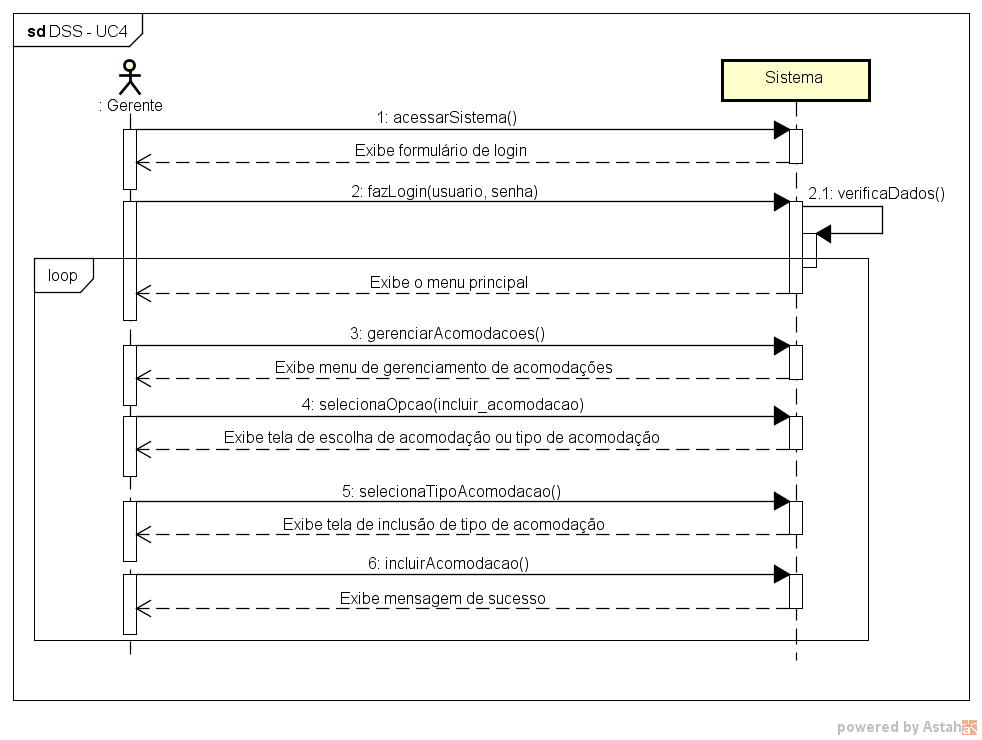
\includegraphics[scale=0.65]{UC4.png}
  \caption{DSS do UC4}
  \label{fig:UC4}
\end{figure}


\clearpage

\section{ID: UC5}
\noindent\textbf{Caso de uso}: Gerenciar Reservas.\\
\textbf{Atores Primários}: Cliente. \\
\textbf{Atores Secundários}: Funcionário do Hotel.\\
\textbf{Propósito}: Incluir, Alterar ou Remover Reservas no Hotel.\\
\textbf{Visão Geral}: O Funcionário do Hotel acessa um painel onde pode incluir, alterar ou remover dados de reserva.\\
\textbf{Pré-condições}: O Funcionário do Hotel já estar cadastrado no sistema.\\
\textbf{Pós-condições}: Uma nova reserva é incluída, removida ou alterada no sistema.\\
\textbf{Referências Cruzadas}: R.6, R.20, R.21, R.22, R.23\\
\newline
\textbf{Fluxo Principal}:\\

\begin{table}[!htbp]
\centering
\label{UC5}
\resizebox{\textwidth}{!}{%
\begin{tabular}{|p{8cm}|p{8cm}|}
\hline
\textbf{Ação do Ator}                                      & \textbf{Resposta do Sistema}                                                                           \\ \hline
1. O Funcionário do Hotel acessa o sistema.                & 2. Exibe tela de login, solicitando email e senha do Funcionário do Hotel.                           \\ \hline
3. O Funcionário do Hotel insere seu email e senha.        & 4. Verifica os dados de login.                                                                         \\ \hline
                                                           & 5. Exibe o Menu Principal.                                                                             \\ \hline
6. O Funcionário do Hotel seleciona a opção “Gerenciar Reservas”.
    & 7. Exibe a tela com as opções Incluir, Alterar ou Remover Reservas. \\ \hline
8. O Funcionário do Hotel seleciona a opção “Incluir”.     & 9. Exibe a tela de inclusão de dados de reserva, com campos de preenchimento específicos.             \\ \hline
10. O Funcionário do Hotel preenche os campos com dados da reserva, como especificado no requisito 5. & 11. Exibe a tela informando que a operação foi realizada com sucesso.                                  \\ \hline
                                                           & 12. Exibe o Menu Principal novamente (Passo 5).                                                        \\ \hline
\end{tabular}%
}
\end{table}

\textbf{Fluxos Alternativos}:\\
\begin{itemize}
\item \underline{Passo 2}: O Funcionário do Hotel já está logado, então avança para o Passo 5.
\item \underline{Passo 4}: O Funcionário do Hotel insere email e/ou senha incorretos. O sistema exibe a tela informando que os dados de login são inválidos, então retorna para o Passo 2.
\item \underline{Passos 2 - 10}: O Funcionário do Hotel deseja encerrar o sistema e cancelar a operação atual, selecionando a opção de fechar o navegador. O sistema é encerrado e nenhuma informação é salva.  
\item \underline{Passos 8 - 10}: O Funcionário do Hotel seleciona a opção “Remover”. O sistema exibe uma tela com as reservas que podem ser removidas e  sistema veifica se a remoção está sendo feita antes de 12 horas do início da reserva. Em caso afirmativo os dados da reserva são deletados do sistema. Em caso negativo, uma mensagem de erro é exibida na tela e retorna ao Passo 5.    
\item \underline{Passos 8 - 10}: O Funcionário do Hotel seleciona a opção “Alterar”. O sistema exibe as reservas que podem ser alteradas. O Funcionário do Hotel seleciona os dados a serem alterados, modifica-os e então clica em "Salvar". Os dados da reserva são atualizados no sistema. 
\item \underline{Passo 10}: O Funcionário do Hotel não preenche todos os dados obrigatórios. O sistema exibe na tela a informação de quais dados estão faltando, então retorna para o Passo 8.
\item \underline{Passo 10}: O sistema verifica que a reserva ou acomodação nos dias selecionados já está ocupada; o sistema informa que a reserva não pode ser efetuada e volta para o Passo 8.
\end{itemize}

\begin{figure}[!htbp]
	\centering
  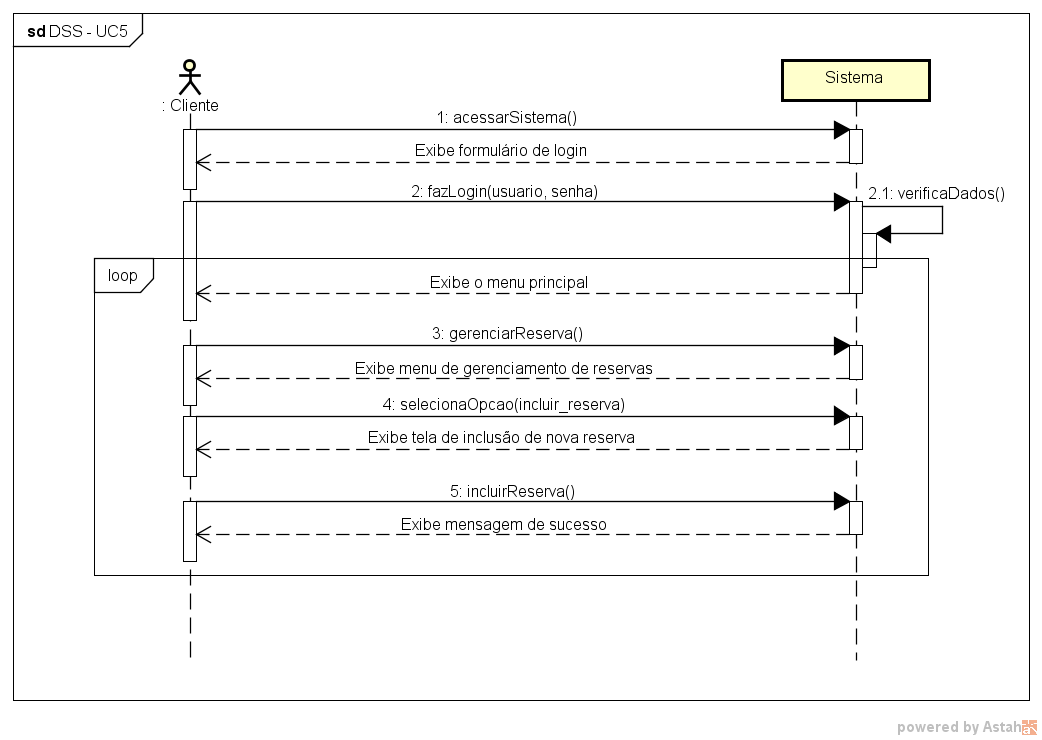
\includegraphics[scale=0.65]{UC5.png}
  \caption{DSS do UC5}
  \label{fig:UC5}
\end{figure}


\clearpage

\section{ID: UC6}
\noindent\textbf{Caso de uso}: Gerenciar Consumo do Hóspede.\\
\textbf{Atores Primários}: Cliente. \\
\textbf{Atores Secundários}: Funcionário do Hotel.\\
\textbf{Propósito}: Incluir, Alterar ou Remover itens consumidos pelo hóspede.\\
\textbf{Visão Geral}: O Funcionário do Hotel acessa um painel onde pode incluir, alterar ou remover itens consumidos pelo hóspede.\\
\textbf{Pré-condições}: O Funcionário do Hotel e o item já estarem cadastrados no sistema.\\
\textbf{Pós-condições}: As informações sobre os itens de consumo do hóspede são atualizadas.\\
\textbf{Referências Cruzadas}: R.8, R.20, R.21, R.22, R.23\\
\newline
\textbf{Fluxo Principal}:\\

\begin{table}[!htbp]
\centering
\label{UC6}
\resizebox{\textwidth}{!}{%
\begin{tabular}{|p{8cm}|p{8cm}|}
\hline
\textbf{Ação do Ator}                                      & \textbf{Resposta do Sistema}                                                                           \\ \hline
1. O Funcionário do Hotel acessa o sistema.                & 2. Exibe tela de login, solicitando email e senha do Funcionário do Hotel.                           \\ \hline
3. O Funcionário do Hotel insere seu email e senha.        & 4. Verifica os dados de login.                                                                         \\ \hline
                                                           & 5. Exibe o Menu Principal.                                                                             \\ \hline
6. O Funcionário do Hotel seleciona a opção “Gerenciar Consumo do Hóspede”.
    & 7. Exibe o menu de gerenciamento de itens de consumo mostrando todos os hóspedes do hotel. \\ \hline
8. O Funcionário do Hotel seleciona o Hóspede em específico.     & 9. Exibe a tela de itens consumidos pelo cliente até o momento e mostra as opções Incluir, Alterar e Remover itens.             \\ \hline
10. O Funcionário do Hotel seleciona a opção “Incluir”.	& 11. Exibe a tela de inclusão de itens de consumo, com seus campos de informações específicos.                                  \\ \hline
 12. O Funcionário do Hotel seleciona os itens pedidos pelo hóspede e preenche as informações necessárias como especificado nos requisitos 2 e 8                                                          & 13. Exibe a tela informando que a operação foi realizada com sucesso.                                            \\ \hline
  & 14. Exibe o Menu Principal novamente (Passo 5). 
 	\\ \hline
\end{tabular}%
}
\end{table}


\textbf{Fluxos Alternativos}:\\
\begin{itemize}
\item \underline{Passo 2}: O Funcionário do Hotel já está logado, então avança para o Passo 5.
\item \underline{Passo 4}: O Funcionário do Hotel insere email e/ou senha incorretos. O sistema exibe a tela informando que os dados de login são inválidos, então retorna para o Passo 2.
\item \underline{Passos 2 - 12}: O Funcionário do Hotel deseja encerrar o sistema e cancelar a operação atual, selecionando a opção de fechar o navegador. O sistema é encerrado e nenhuma informação é salva.  
\item \underline{Passos 10 - 12}:  O Funcionário do Hotel seleciona os itens de consumo a serem removidos e clica na opção “Remover”; o sistema deleta os dados dos itens de consumo selecionados do sistema e atualiza a página de itens de consumo. 
\item \underline{Passos 10 - 12}: O Funcionário do Hotel seleciona os itens de consumo a serem alterados e clica na opção “Alterar”; o sistema exibe uma página de edição dos itens de consumo e o Funcionário do Hotel modifica as informações dos itens. O sistema então salva as novas informações sobre os itens de consumo e atualiza a página de itens de consumo.
\item \underline{Passo 13}: O sistema verifica que não há unidades suficientes do item pedido então emite um aviso para o Funcionário do Hotel e volta para a tela de inclusão de itens (Passo 11).

\end{itemize}

\begin{figure}[!htbp]
	\centering
  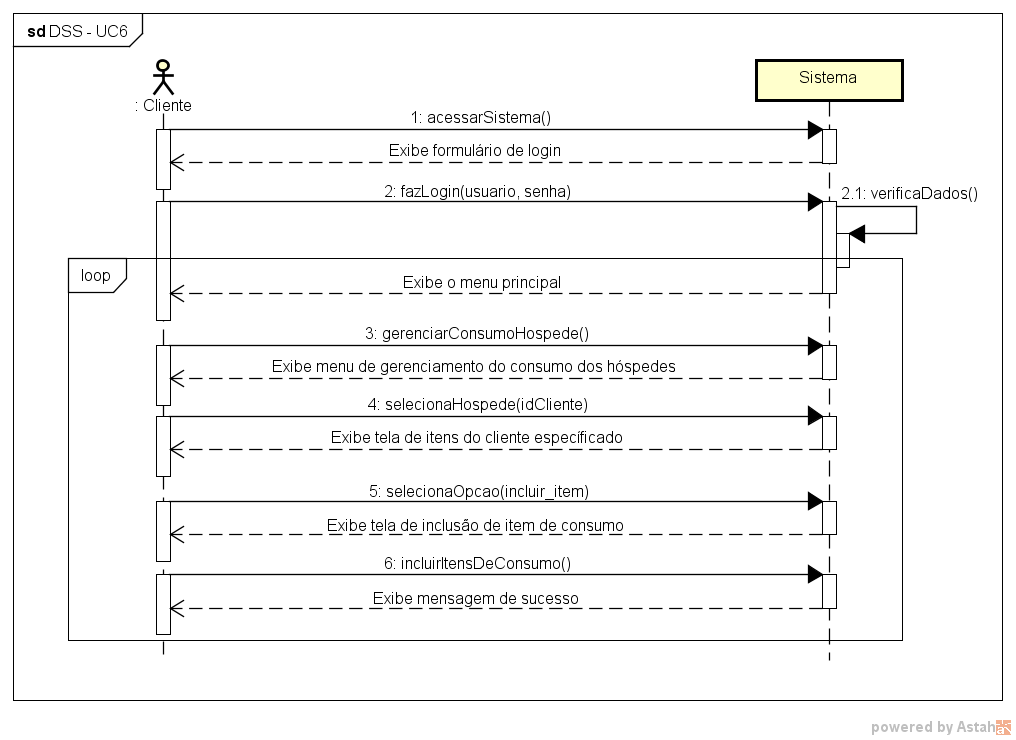
\includegraphics[scale=0.65]{UC6.png}
  \caption{DSS do UC6}
  \label{fig:UC6}
\end{figure}

\clearpage

\section{ID: UC7}
\noindent\textbf{Caso de uso}: Efetuar Pagamento.\\
\textbf{Atores Primários}: Cliente. \\
\textbf{Atores Secundários}: Funcionário do Hotel.\\
\textbf{Propósito}: Efetuar pagamento referente à reserva do cliente.\\
\textbf{Visão Geral}: O hotel recebe o pagamento pela reserva do cliente.\\
\textbf{Pré-condições}: O Funcionário do Hotel já estar cadastrado no sistema. Além disso, o cliente deve ter realizado uma reserva e o hotel deve ter registrado os gastos do cliente durante sua estadia.\\
\textbf{Pós-condições}: As dívidas do cliente com o hotel são dadas como quitadas no sistema, e os dados dessas estadia são registrados no histórico do hotel.\\
\textbf{Referências Cruzadas}: R.9, R.10, R.11, R.20, R.21, R.22, R.23\\
\newline
\textbf{Fluxo Principal}:\\

\begin{table}[!htbp]
\centering
\label{UC7}
\resizebox{\textwidth}{!}{%
\begin{tabular}{|p{8cm}|p{8cm}|}
\hline
\textbf{Ação do Ator}                                      & \textbf{Resposta do Sistema}                                                                           \\ \hline
1. O Funcionário do Hotel acessa o sistema.                & 2. Exibe tela de login, solicitando email e senha do Funcionário do Hotel.                           \\ \hline
3. O Funcionário do Hotel insere seu email e senha.        & 4. Verifica os dados de login.                                                                         \\ \hline
                                                           & 5. Exibe o Menu Principal.                                                                             \\ \hline
6. O Funcionário do Hotel seleciona a opção “Receber Pagamento do Cliente”.
    & 7. Solicita os dados da reserva. \\ \hline
8. O Funcionário do Hotel insere os dados da reserva.     & 9. Procura pelos dados da reserva e atividades do cliente dentro do hotel.             \\ \hline
	& 10. Exibe o preço a ser pago. \\ \hline
11. O Funcionário do Hotel confirma o pagamento do cliente. & 11. Exibe a tela informando que a operação foi realizada com sucesso.                                  \\ \hline
                                                           & 12. Exibe o Menu Principal novamente (Passo 5).                                                        \\ \hline
\end{tabular}%
}
\end{table}

\textbf{Fluxos Alternativos}:\\
\begin{itemize}
\item \underline{Passo 2}: O Funcionário do Hotel já está logado, então avança para o Passo 5.
\item \underline{Passo 4}: O Funcionário do Hotel insere email e/ou senha incorretos. O sistema exibe a tela informando que os dados de login são inválidos, então retorna para o Passo 2.
\item \underline{Passos 2 - 9}: O Funcionário do Hotel deseja encerrar o sistema e cancelar a operação atual, selecionando a opção de fechar o navegador. O sistema é encerrado e nenhuma informação é salva.  
\item \underline{Passo 9}: Os dados inseridos estão errados e o sistema não encontra a reserva. Volta para o Passo 7.
\end{itemize}

\begin{figure}[!htbp]
	\centering
  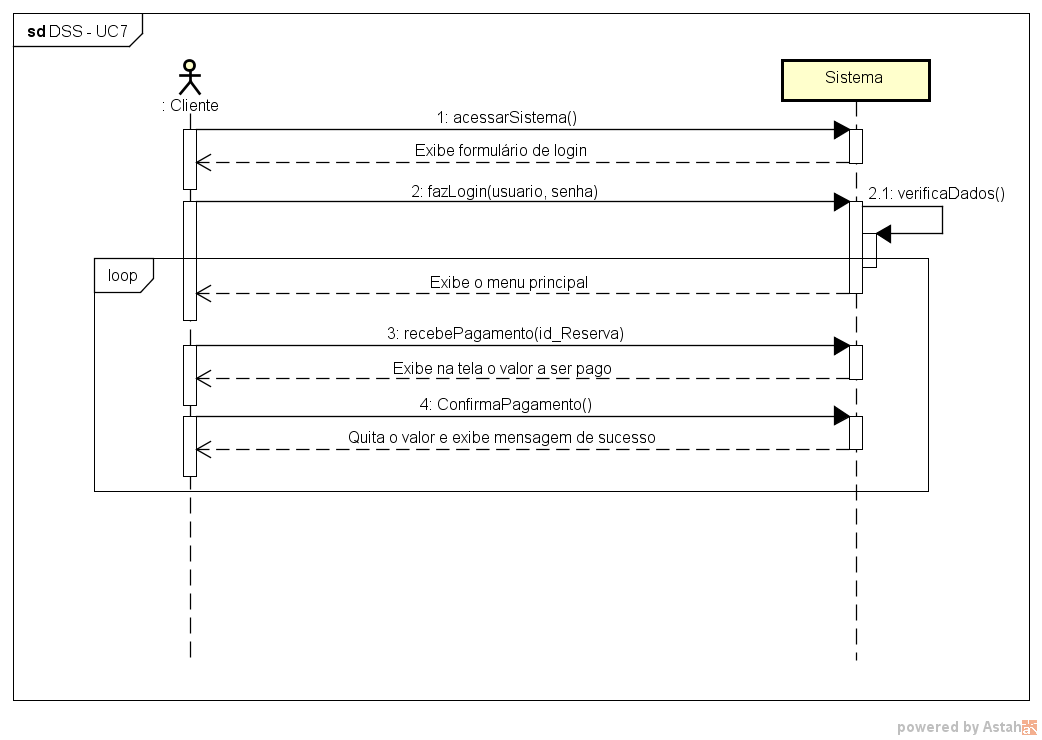
\includegraphics[scale=0.65]{UC7.png}
  \caption{DSS do UC7}
  \label{fig:UC7}
\end{figure}

\clearpage

\section{ID: UC8}
\noindent\textbf{Caso de uso}: Imprimir Histórico de Estadias no Hotel.\\
\textbf{Atores Primários}: Funcionário do Hotel. \\
\textbf{Atores Secundários}: \\
\textbf{Propósito}: Efetuar a impressão dos dados, na tela, de estadia dos hóspedes.\\
\textbf{Visão Geral}: O Funcionário do Hotel acessa o painel e recebe o histórico de estadias impresso na tela.\\
\textbf{Pré-condições}: O Funcionário do Hotel já estar cadastrado no sistema.\\
\textbf{Pós-condições}: Nenhuma.\\
\textbf{Referências Cruzadas}: R.12, R.20, R.21, R.22, R.23, R.24\\
\newline
\textbf{Fluxo Principal}:\\

\begin{table}[!htbp]
\centering
\label{UC8}
\resizebox{\textwidth}{!}{%
\begin{tabular}{|p{8cm}|p{8cm}|}
\hline
\textbf{Ação do Ator}                                      & \textbf{Resposta do Sistema}                                                                           \\ \hline
1. O Funcionário do Hotel acessa o sistema.                & 2. Exibe tela de login, solicitando email e senha do Funcionário do Hotel.                           \\ \hline
3. O Funcionário do Hotel insere seu email e senha.        & 4. Verifica os dados de login.                                                                         \\ \hline
                                                           & 5. Exibe o Menu Principal.                                                                             \\ \hline
6. O Funcionário do Hotel seleciona a opção “Imprimir Histórico de Estadias no Hotel”.
    & 7. Exibe o Histórico de Estadias no Hotel. \\ \hline
    8. O Funcionário do Hotel clica em "Fechar". & 9. Exibe o Menu Principal novamente (Passo 5).                                                        \\ \hline
\end{tabular}%
}
\end{table}

\textbf{Fluxos Alternativos}:\\
\begin{itemize}
\item \underline{Passo 2}: O Funcionário do Hotel já está logado, então avança para o Passo 5.
\item \underline{Passo 4}: O Funcionário do Hotel insere email e/ou senha incorretos. O sistema exibe a tela informando que os dados de login são inválidos, então retorna para o Passo 2.
\item \underline{Passos 2 - 6}: O Funcionário do Hotel deseja encerrar o sistema e cancelar a operação atual, selecionando a opção de fechar o navegador. O sistema é encerrado e nenhuma informação é salva.  
\end{itemize}
\begin{figure}[!htbp]
	\centering
  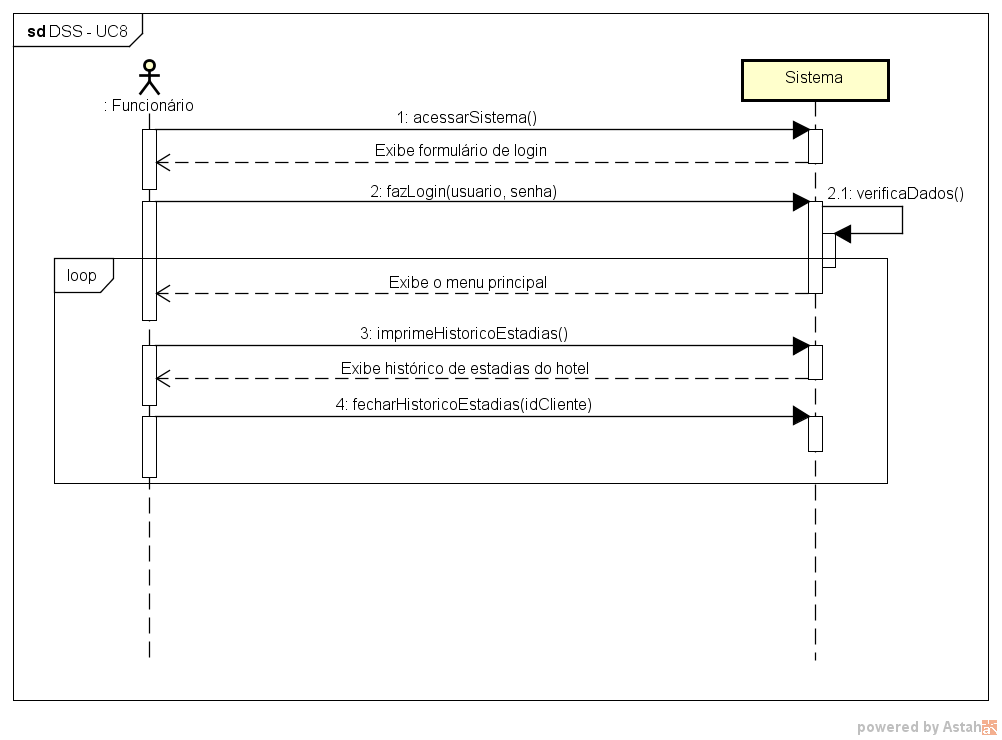
\includegraphics[scale=0.65]{UC8.png}
  \caption{DSS do UC8}
  \label{fig:UC8}
\end{figure}

\clearpage

\section{ID: UC9}
\noindent\textbf{Caso de uso}: Imprimir Comprovante de Saída do Hóspede.\\
\textbf{Atores Primários}: Cliente. \\
\textbf{Atores Secundários}: Funcionário do Hotel.\\
\textbf{Propósito}: Imprimir um comprovante de saída para o cliente.\\
\textbf{Visão Geral}: O Funcionário do Hotel imprime um comprovante de saída para o cliente.\\
\textbf{Pré-condições}: O cliente deve estar realizando a saída do hotel, o cliente deve ter quitado a reservar e o Funcionário do Hotel deve estar cadastrado no sistema.\\
\textbf{Pós-condições}: Nenhuma.\\
\textbf{Referências Cruzadas}: R.14, R.20, R.21, R.22, R.23, R.24, UC1\\
\newline
\textbf{Fluxo Principal}:\\

\begin{table}[!htbp]
\centering
\label{UC9}
\resizebox{\textwidth}{!}{%
\begin{tabular}{|p{8cm}|p{8cm}|}
\hline
\textbf{Ação do Ator}                                      & \textbf{Resposta do Sistema}                                                                           \\ \hline
1. O Funcionário do Hotel acessa o sistema.                & 2. Exibe tela de login, solicitando email e senha do Funcionário do Hotel.                           \\ \hline
3. O Funcionário do Hotel insere seu email e senha.        & 4. Verifica os dados de login.                                                                         \\ \hline
                                                           & 5. Exibe o Menu Principal.                                                                             \\ \hline
6. O Funcionário do Hotel seleciona a opção “Gerenciar Hóspedes”.
    & 7. Exibe a tela com as opções Incluir, Alterar, Remover, Fazer Check-in e Fazer Check-out de Clientes. \\ \hline
    8. O Funcionário do Hotel seleciona a opção “Checkout de Clientes”. & 9. Exibe a tela mostrando Clientes que quitaram sua reserva porém ainda não tiveram o comprovante impresso.                                                        \\ \hline
    10. O Funcionário do Hotel seleciona o Cliente que está realizando a saída e pressiona no botão “Imprimir Comprovante”. & 11. Imprime o Comprovante Físico para o Funcionário do Hotel entregar ao Cliente. \\ \hline
     & 12. Exibe o Menu Principal novamente (Passo 5). \\ \hline
    
\end{tabular}%
}
\end{table}

\textbf{Fluxos Alternativos}:\\
\begin{itemize}
\item \underline{Passo 2}: O Funcionário do Hotel já está logado, então avança para o Passo 5.
\item \underline{Passo 4}: O Funcionário do Hotel insere email e/ou senha incorretos. O sistema exibe a tela informando que os dados de login são inválidos, então retorna para o Passo 2.
\item \underline{Passos 2 - 10}: O Funcionário do Hotel deseja encerrar o sistema e cancelar a operação atual, selecionando a opção de fechar o navegador. O sistema é encerrado e nenhuma informação é salva.  
\item \underline{Passos 6, 8, 10}:O Funcionário do Hotel decide cancelar a operação; retorna ao Passo 5.
\item \underline{Passo 11}: O sistema não detecta uma impressora. O sistema anuncia que não encontra hardware para impressão e aguarda até que um seja inserido no aparelho ou a operação seja cancelada.
\end{itemize}

\begin{figure}[!htbp]
	\centering
  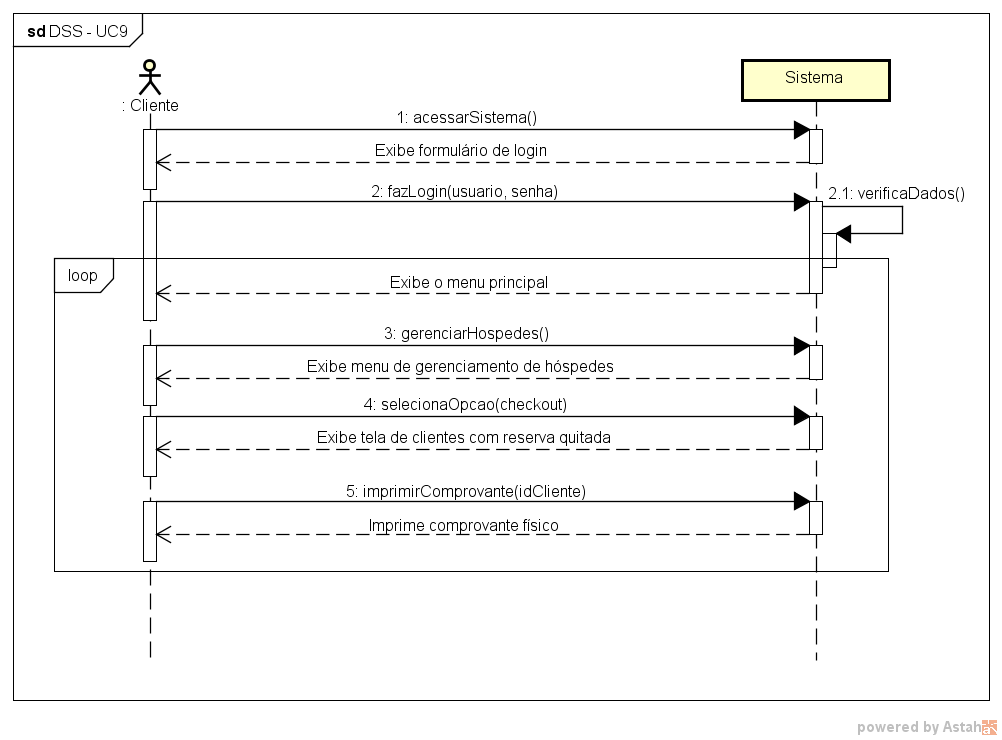
\includegraphics[scale=0.65]{UC9.png}
  \caption{DSS do UC9}
  \label{fig:UC9}
\end{figure}

\clearpage

\section{ID: UC10}
\noindent\textbf{Caso de uso}: Imprimir Informações para Hotel.\\
\textbf{Atores Primários}: Funcionário do Hotel. \\
\textbf{Atores Secundários}: \\
\textbf{Propósito}: Imprimir dados, na tela, referentes ao gerenciamento do hotel.\\
\textbf{Visão Geral}: O Funcionário do Hotel deve acessar um painel que o permita imprimir informações pertinentes ao gerenciamento do hotel, entre elas reservas, contas e pagamentos.\\
\textbf{Pré-condições}: O Funcionário do Hotel deve estar cadastrado no sistema.\\
\textbf{Pós-condições}: Nenhuma.\\
\textbf{Referências Cruzadas}: R.13, R.16, R.17, R.18, R.19, R.20, R.21, R.22, R.23, R.24\\
\newline
\textbf{Fluxo Principal}:\\

\begin{table}[!htbp]
\centering
\label{UC10}
\resizebox{\textwidth}{!}{%
\begin{tabular}{|p{8cm}|p{8cm}|}
\hline
\textbf{Ação do Ator}                                      & \textbf{Resposta do Sistema}                                                                           \\ \hline
1. O Funcionário do Hotel acessa o sistema.                & 2. Exibe tela de login, solicitando email e senha do Funcionário do Hotel.                           \\ \hline
3. O Funcionário do Hotel insere seu email e senha.        & 4. Verifica os dados de login.                                                                         \\ \hline
                                                           & 5. Exibe o Menu Principal.                                                                             \\ \hline
6. O Funcionário do Hotel seleciona a opção “Imprimir Informações Gerenciais”.
    & 7. Retorna o painel de informações gerenciais. \\ \hline
    8. O Funcionário do Hotel seleciona a opção “Imprimir Informações Pertinentes ao Gerenciamento do Hotel”. & Exibe as reservas, contas e pagamentos do hotel. \\ \hline
    & 10. Exibe o Menu Principal novamente (Passo 5). \\ \hline
    
\end{tabular}%
}
\end{table}

\textbf{Fluxos Alternativos}:\\
\begin{itemize}
\item \underline{Passo 2}: O Funcionário do Hotel já está logado, então avança para o Passo 5.
\item \underline{Passo 4}: O Funcionário do Hotel insere email e/ou senha incorretos. O sistema exibe a tela informando que os dados de login são inválidos, então retorna para o Passo 2.
\item \underline{Passos 2 - 9}: O Funcionário do Hotel deseja encerrar o sistema e cancelar a operação atual, selecionando a opção de fechar o navegador. O sistema é encerrado e nenhuma informação é salva.  
\end{itemize}
\begin{figure}[!htbp]
	\centering
  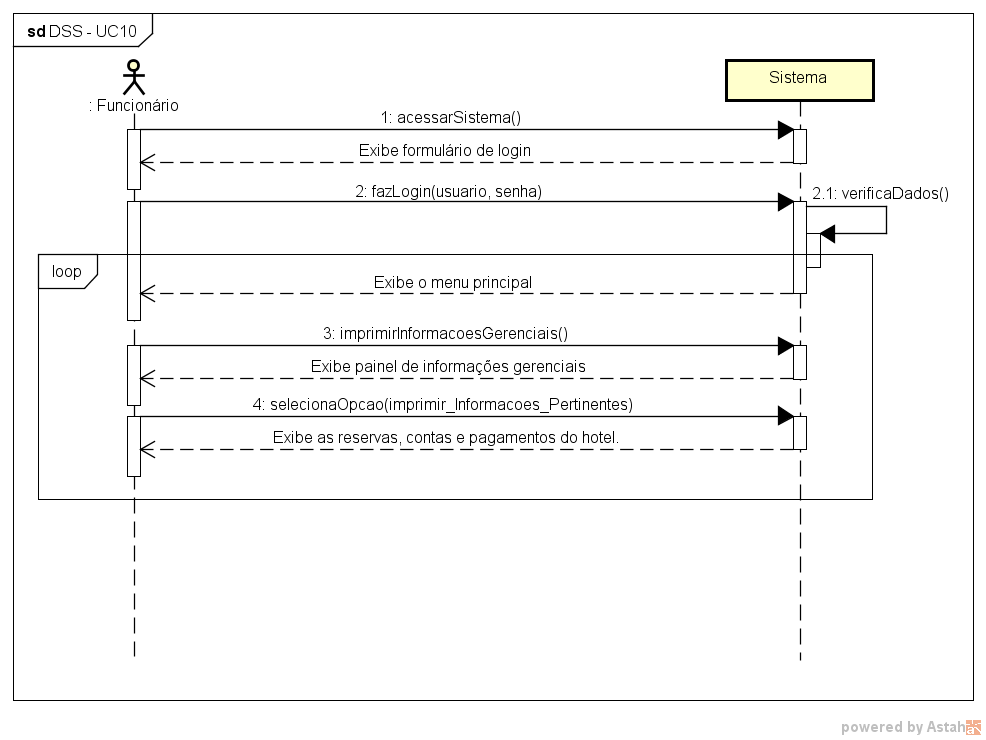
\includegraphics[scale=0.65]{UC10.png}
  \caption{DSS do UC10}
  \label{fig:UC10}
\end{figure}

\clearpage

\section{ID: UC11}
\noindent\textbf{Caso de uso}: Imprimir Histórico de Estadia do Hóspede.\\
\textbf{Atores Primários}: Cliente. \\
\textbf{Atores Secundários}: \\
\textbf{Propósito}: Imprimir dados, na tela, referentes às estadias anteriores do cliente no hotel.\\
\textbf{Visão Geral}: O cliente deve acessar o painel que o permite imprimir informações pertinentes ao histórico de estadia no hotel, entre elas data de entrada e saída e os valores pagos em cada ocasião.\\
\textbf{Pré-condições}: O cliente deve estar cadastrado e portar um senha de acesso.\\
\textbf{Pós-condições}: Nenhuma.\\
\textbf{Referências Cruzadas}:R.15, R.20, R.21, R.22, R.23, R.24\\
\newline
\textbf{Fluxo Principal}:\\

\begin{table}[!htbp]
\centering
\label{UC10}
\resizebox{\textwidth}{!}{%
\begin{tabular}{|p{8cm}|p{8cm}|}
\hline
\textbf{Ação do Ator}                                      & \textbf{Resposta do Sistema}                                                                           \\ \hline
1. O Cliente do Hotel acessa o sistema.                & 2. Exibe tela de login, solicitando email e senha do Cliente do Hotel.                           \\ \hline
3. O Cliente do Hotel insere seu email e senha.        & 4. Verifica os dados de login.                                                                         \\ \hline
                                                           & 5. Exibe o Menu Principal.                                                                             \\ \hline
6. O Cliente do Hotel seleciona a opção “Imprimir Histórico de Estadia”.
    & 7. Imprime, na tela, as informações. \\ \hline
   & 8. Exibe o Menu Principal novamente (Passo 5). \\ \hline
    
\end{tabular}%
}
\end{table}

\textbf{Fluxos Alternativos}:\\
\begin{itemize}
\item \underline{Passo 2}: O Cliente do Hotel já está logado, então avança para o Passo 5.
\item \underline{Passo 4}: O Cliente do Hotel insere email e/ou senha incorretos. O sistema exibe a tela informando que os dados de login são inválidos, então retorna para o Passo 2.
\item \underline{Passos 2 - 7}: O Cliente do Hotel deseja encerrar o sistema e cancelar a operação atual, selecionando a opção de fechar o navegador. O sistema é encerrado e nenhuma informação é salva.  
\end{itemize}
\begin{figure}[!htbp]
	\centering
  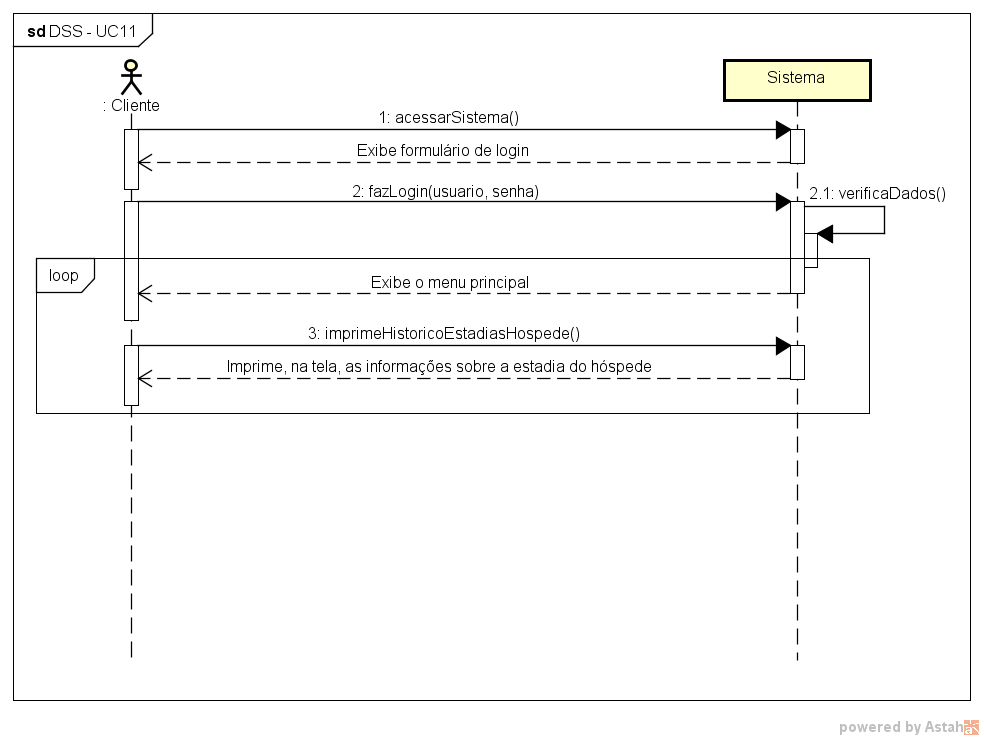
\includegraphics[scale=0.65]{UC11.png}
  \caption{DSS do UC11}
  \label{fig:UC11}
\end{figure}

\clearpage
\tableofcontents

\end{document}


